\documentclass[a4paper]{article}
\usepackage[utf8]{inputenc}
\usepackage[margin=50pt]{geometry}
\usepackage{tabulary}
\usepackage{graphicx}
\usepackage{xcolor}


\title{Ingegneria del Software T}
\author{
    Luca Bartolomei 
    \texttt{0000825005}
    \\
    Luigi Di Nuzzo
    \texttt{0000824873}
    \\
    Filippo Veronesi
    \texttt{0000832244}
}

\date{Marzo 2020}

\begin{document}

\maketitle

\tableofcontents

\newpage

\section{Abstract}

Il progetto riguarda la creazione di un applicativo software gestionale per prevendite elettroniche.\\
Abbiamo pensato il software per un gruppo di amici che organizzano feste, con obiettivi cardine l'abbattimento di costi, l'ottimizzazione dell'entrata dei partecipanti all'evento e una semplificazione dei conti di bilancio.\\
L'idea di fondo è di utilizzare, come sostitutivo alla prevendita cartacea, un codice QR in grado di far entrare il cliente dopo relativo check all'entrata.\\
Il risparmio economico ottenuto è ovviamente importante in confronto alla vendita tradizionale. Tuttavia bisogna tenere in conto dei problemi tecnologici che si possono verificare durante la vendita e l'entrata: problemi di connessione Internet, incompatibilità dei dispositivi dei clienti, training del personale addetto alle entrate, eccetera.\\
Viene gestito oltre alle prevendite e relatvi clienti, anche l'organizzazione e i vari membri dell'organizzazione, con divisione dei ruoli.\\
Per facilitare i conti di bilancio è disponibile una sezione in cui è possibile ricavare statistiche sull'andamento dell'evento.

\section{Analisi dei requisiti}

\subsection{Requisiti del sistema}

\begin{itemize}
	
	\item \textbf{REQUISITI FUNZIONALI}
		
	\item R1F - Il software prevede la possibilità di gestire più staff.
	
	%-Requisiti di sicurezza
	
	%--Requisiti di identificazione
	\item R2F - Gli utenti devono essere identificati tramite username.
	
	%--Requisito di autenticazione
	\item R3F - Gli utenti sono autenticati tramite credenziali di username e password.
	\item R4F - L'accesso ad uno staff, da parte di un utente, avviene tramite codice di accesso.	

	%Funzionale/non funzionale
	\item R5F - La registrazione di utenti è a carico dell'amministratore di sistema.
	\item R6F - Possibilità di cambiare la password personale dell'utente.
		
	%--Requisiti di Autorizzazione
	\item R7F - Ogni membro di uno staff può ricoprire dei ruoli: cassiere, PR, amministratore.	
	\item R8F - Il ruolo di cassiere riguarda la timbratura di prevendite all'ingresso di un evento.
	\item R9F - Il ruolo di PR riguarda la vendita di prevendite a clienti.
	\item R10F - Il ruolo di amministratore riguarda la gestione dei membri, degli eventi, delle tipologie di prevendita di un evento e della visualizzazione di tutte statistiche.
	
	%--Requisiti di scoperta alle intrusioni
	\item R11F - Utilizzo di log per monitorare operazioni critiche.

	%--Requisiti di riservatezza
	\item R12F - Le password devono essere salvate in modo sicuro.
	
	%Non vuol dire cifrato! Basta un controllo agli accessi.
	%Se salvi in DB ricorda di indicizzare.
	%\item Il log deve essere salvato in modo abbastanza sicuro.
	
	%--------------------
	
	%Accesso e creazione di uno staff
	\item R13F - Ogni utente registrato nel gestionale può diventare membro di uno o più staff. 
	
	\item R14F - Quando un utente crea uno staff ne diventa membro e amministratore.
	
	%Timbratura (Cassiere)
	\item R15F - La timbratura di una prevendita valida permette al cliente di entrare all'evento, ovviamente lo staff potrà effettuare ulteriori controlli non previsti dal sistema e decidere di far entrare un cliente.
	
	
	%Non viene specificata la modalità di consegna: URL, file immagine file testo etc.
	\item R16F - La vendita di una prevendita elettronica consiste nella consegna al cliente di un documento digitale di qualche forma, associato alla prevendita elettronica venduta.

	
	%Gestione staff (Amministratore)
	\item R17F - Un amministratore può concedere/revocare i ruoli a qualsiasi membro dello staff. Unico vincolo è che rimanga almeno un amministratore.
	\item R18F - Possibilità di cambiare il codice di accesso dello staff da parte di un amministratore.
	   
	\item R19F - Per gestione degli eventi di uno staff si intende la possibilità di vedere gli staff di un evento, di creane uno nuovo e di poter modificare un evento dello staff.
		
	\item R20F - La gestione delle tipologie di prevedita di un evento indica l'aggiunta, la modifica e la rimozione delle tipologie di prevendita.
	
	%Definizioni
	%-Eventi
	\item R21F - Un evento è composto da un nome, una descrizione, un periodo temporale di svolgimento e un luogo. 
	\item R22F - Un evento può essere annullato, anche se ci sono prevendite vendute.
	
	%Tipologia Prevendita
	\item R23F - Una tipologia di prevendita serve ad associare alla prevendita un prezzo, una descrizione e un periodo di vendita a tutte le prevendite con la stessa tipologia.

	%-Prevendite
	\item R24F - Una prevendita può essere annullata e/o rimborsata. 
	
	%-Statistiche
	\item R25F - Le statistiche di un membro sono suddivise per ruolo coperto all'interno dello staff: cassiere o PR.
	
	\item R26F - Lo sblocco dell'utente è a carico dell'amministratore di sistema.
	
	%Si deduce dalla precedente
	%\item Il ruolo di amministratore non prevede statistiche personali.
		
    \item \textbf{REQUISITI NON FUNZIONALI}
	
	%Se si verifica attacco freezing dell'account cambiare username.
	\item R1NF - Il blocco dell'account deve avvenire dopo 3 tentativi.
	
	\item R2NF - La password degli utenti deve essere lunga almeno 8 caratteri.
	\item R3NF - Il codice di accesso allo staff deve essere lungo almeno 4 caratteri.
	\item R4NF - Ogni utente registrato può creare al massimo uno staff.
	\item R5NF - Requisito fondamentale è il basso costo del prodotto software.
	\item R6NF - Utilizzare uno o più metodi per velocizzare l'autenticazione dell'utente.
	\item R7NF - I membri non amministratori possono vedere solo le statistiche personali.	
	\item R8NF - I membri non amministratori possono solo vedere le tipologie di prevendite associate ad un evento.
	\item R9NF - I membri non amministratori possono solo vedere gli eventi dello staff.
	\item R10NF - Il periodo di vendita delle prevendite deve essere antecedente il periodo dell'evento.
	\item R11NF - Una prevendita annullata e/o rimborsata rimane tale.
	\item R12NF - Un evento annullato rimane tale.
	\item R13NF - Si prevedono più forme di consegna del documento digitale, per affrontare le eterogeneità.
	\item R14NF - Il documento digitale consegnato al cliente sarà utilizzato dal cassiere all'ingresso timbrare la prevedita elettronica.
	\item R15NF - La password fornita dall'amministratore di sistema a tempo di registrazione va cambiata immediatamente dopo il login.
	
	%Devo contare i tentativi falliti nel db: nella sessione potrei cancellare i cookie.
	\item R16NF - Bloccare l'account utente dopo troppi tentativi di accesso e notificarlo nei log.
	
	\item R17NF - Ogni ruolo è indipendente.
	\item R18NF - Ogni staff gestito dal software è indipendente.
	
	%Utilizzo https per la cifratura
	\item R19NF - Si richiede una comunicazione sicura.
	
	%Sistema locale senza server remoto tramite server locale + wifi
	\item R20NF - Si richiedono procedure manuali o automatiche per cercare di garantire la disponibilità del servizio.
	
	%Codice della prevendita
	%Prevendita nominativa
	\item R21NF - Si richiedono metodi per evitare la contraffazione delle prevendite.
	
	%Log
	\item R22NF - Prevedere livelli di log per aiutare l'analisi da parte dell'amministratore di sistema.
	
	%Prevendita
	\item R23NF - Ogni prevendita venduta è associata ad una sola tipologia di prevendita.
	\item R24NF - La tipologia di prevendita associata non è modificabile.
	\item R25NF - Ogni prevedita è nominativa.
	
	%Tipologia prevendita
	\item R26NF - Il prezzo di una tipologia di prevendita è modificabile solo se non sono state vendute prevendite con quella determinata tipologia.
	
	%--Requisiti di non-ripudiabilità
	\item R27NF - Quando un PR vende una prevendita, essa viene associata ad esso.
	\item R28NF - Quando un Cassiere timbra una prevendita, essa viene associata ad esso.
	
	%Vendita (PR)
	\item R29NF - Prima della vendita il cliente sceglierà una tipologia di prevendita associata all'evento a cui vuole partecipare.
	
	\item R30NF - La timbratura può essere fatta solo una volta.
	
	
\end{itemize}

\newpage

\subsection{Analisi del dominio}

\subsubsection{Glossario}

\begin{table}[ht!]
  \begin{center}
    \begin{tabulary}{1\textwidth}{c|C|C}
        \textbf{Voce} & \textbf{Definizione} & \textbf{Sinonimi}\\
        \hline
        \hline
		Amministratore di sistema & Utente con privilegi di sistema aggiuntivi. & \\
		\hline
		Privilegio di sistema & Autorizzazione intrinseca concessa ad un amministratore di sistema che riguarda la gestione del software stesso. Non riguarda gli staff. & \\
		\hline
        Staff & Gruppo di utenti con lo scopo di organizzare eventi. & Ente organizzatore \\
        \hline
        Utente & Persona registrata nel software gestione. & \\
        \hline
		Cliente & Persona che vuole partecipare ad un evento di uno staff & \\
		\hline
        Membro & Utente che è iscritto ad uno staff. & Organizzatore \\
        \hline
		PR & Membro di uno staff che si occupa della vendita di prevendite & \\
		\hline
		Cassiere & Membro di uno staff che si occupa dell'entrata dei clienti ad un evento & \\
		\hline
		Amministratore & Membro di uno staff che si occupa della gestione dello staff steso & \\
		\hline
        Ruolo & Autorizzazione che ha il membro all'interno dello staff & Autorizzazione \\
        \hline
        Evento & Avvenimento registrato dallo staff, per il quale è possibile vendere prevendite e registrare ingressi & Festa \\
        \hline
        Tipologia Prevendita & Modello associato ad un evento, la quale da le caratteristiche di prezzo e descrizione alla prevendita venduta & Tipo Prevendita \\
        \hline
        Prevendita & Biglietto venduto anticipatamente, che consente l'entrata all'evento pagato & Ticket, Prevendita Elettronica \\
        \hline
		Statistiche & Informazioni di carattere gestionale, riguardo ad un evento o a un membro dello staff & \\
		\hline
		Documento digitale & Si tratta di una risorsa digitale, reperibile dal cliente, che serve a identificare una prevendita venduta & \\
		\hline
		Log & Registro dove vengono salvate informazioni per risalire ad operazioni critiche svolte. Composto da una serie di voci & Registro \\
		\hline
		Voce di log & Si tratta di una riga del log. & Record del log\\
		\hline
		Operazione & Comando richiesto al software gestionale da parte di un utente & \\
		\hline
		Login & Operazione per identificare un utente & Accesso utente \\
		\hline
		Timbratura & Operazione svolta da un cassiere svolta per validare una prevendita di un cliente & Convalida della prevendita \\
		\hline
		Credenziali & Coppia di valori username e password utilizzata per l'autenticazione dell'utente & \\
		\hline
		Username & Stringa di caratteri alfanumerici. Serve a identificare l'utente & \\
		\hline
		Password & String di caratteri alfanumerici. Può contenere caratteri speciali. & \\
		\hline
		Periodo di vendita & Periodo temporale in cui la prevendita è vendibile ai clienti & \\
		\hline
    \end{tabulary}
  \end{center}
\end{table}

\newpage

\subsection{Casi d'uso}

%Specificare i casi d'uso?
%Gestione utente: Sblocco utente, Registrazione utente
%Gestione Log: leggi Log, aggiungi log, cancella log
%Gestione vendita prevendita: aggiungi prevendita, annulla prevendita
%Gestione entrata: timbra entrata, leggi prevendita,
%Gestione eventi: aggiungi evento, modifica evento, annulla evento
%Gestione tipologie prevendite: aggiungi tipologia prevendita, modifica tipologia prevendita, elimina tipologia prevendita.
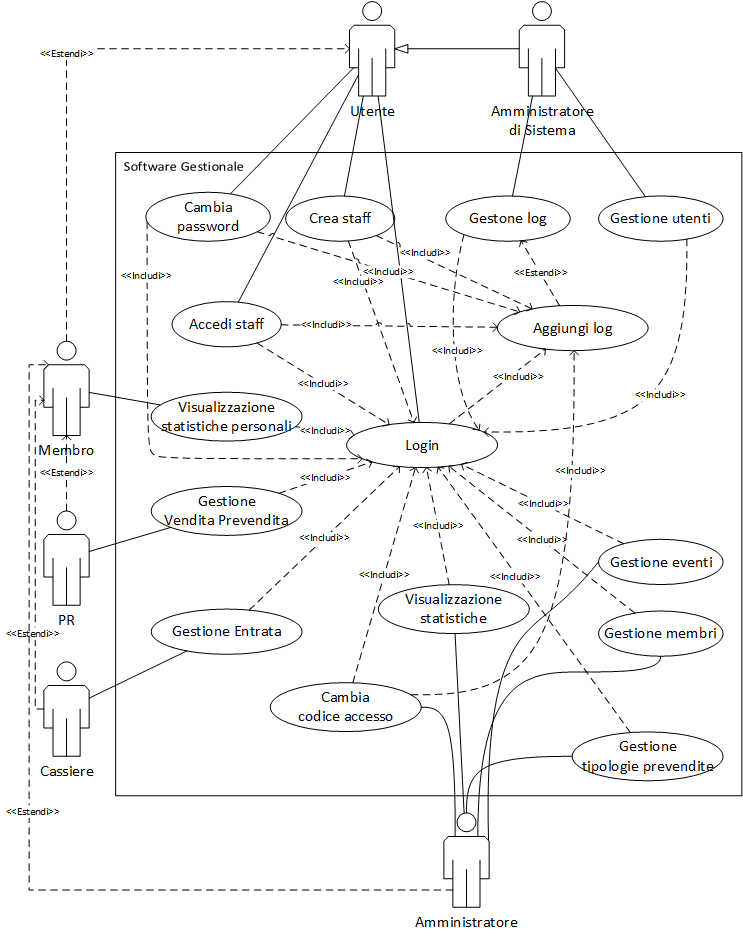
\includegraphics[scale=0.9]{use_cases.png}

L'utilizzo del login (frecce \textcolor{red}{rosse}) è necessario per tutti i servizi forniti agli attori.
Non abbiamo approfondito molo in quanto si avrebbe avuto un diagramma pesante per la lettura.
Tutte le funzioni che abbiamo ritenute critiche utilizzano il caso d'uso "Aggiungi log" (frecce \textcolor{blue}{blu}).
Abbiamo differenziato i casi d'uso delle statistiche perché si tratta di concetti diversi.

\newpage

\subsection{Scenari}

%Login

\begin{table}[ht!]
  \begin{center}
    \begin{tabulary}{1\textwidth}{l|L}
        \textbf{Titolo} & Login \\
        \hline
        \textbf{Descrizione} & Autenticazione nel software gestionale \\
        \hline
        \textbf{Attori} & Utente \\
        \hline
        \textbf{Relazioni} & Aggiungi log, Cambia Password \\
        \hline
        \textbf{Precondizioni} &  \\
        \hline
        \textbf{Postcondizioni} &  \\
        \hline
        \textbf{Scenario principale} & 1. Impostazione di una schermata per l'inserimento di username e password. \\
                                     & 2. L'utente inserisce i dati del proprio account. \\
                                     & 3. L'utente esegue l'operazione. \\
                                     & 4. Il sistema verifica le credenziali. \\
                                     & 5. Dopo l'autenticazione viene mostrata una schermata principale.\\
                                     & 6. Viene notificato l'evento nei log.\\
        \hline
        \textbf{Scenari alternativi} & A) L'utente sbaglia credenziali: \\
                                     & \quad 1. Notifica all'utente.\\
                                     & \quad 2. Ritorno alla schermata di login.\\
                                     & B) L'utente ha sbagliato troppe volte le credenziali: \\
                                     & \quad 1. Blocco dell'account.\\
                                     & \quad 2. Notifica all'utente.\\
                                     & \quad 3. Ritorno alla schermata di login.\\
                                     & C) L'utente ha la password di default impostata dall'amministratore di sistema:\\
                                     & \quad 1. Passaggio al cambio password.\\
        \hline
        \textbf{Requisiti non funzionali} & R1NF, R2NF, R15NF, R16NF \\
        \hline
        \textbf{Punti aperti} & \\
        \hline
    \end{tabulary}
  \end{center}
\end{table}

%Gestione utenti
%Forse da dividere in registrazione utente e sblocco utente

\begin{table}[ht!]
  \begin{center}
    \begin{tabulary}{1\textwidth}{l|L}
        \textbf{Titolo} & Gestione utenti \\
        \hline
        \textbf{Descrizione} & Gestione degli utenti presenti nel software gestionale \\
        \hline
        \textbf{Attori} & Amministratore di sistema, Utente \\
        \hline
        \textbf{Relazioni} & Login \\
        \hline
        \textbf{Precondizioni} &  \\
        \hline
        \textbf{Postcondizioni} &  \\
        \hline
        \textbf{Scenario principale} & 1. Autenticazione tramite login. \\
                                     & 2. L'amministratore di sistema accede alla gestione utenti. \\
                                     & 3. Il sistema fornisce una vista per scegliere tra i comandi. \\
                                     & 4. L'amministratore di sistema sceglie una funzione: \\
                                     & \quad a. Registrazione utente \\
                                     & \quad b. Sblocco utente \\
                                     & 5. L'amministratore di sistema esegue l'operazione, dopo aver consultato l'utente interessato.\\
        \hline
        \textbf{Scenari alternativi} & A) L'utente autenticato non è amministratore di sistema: \\
                                     & \quad 1. Notifica all'utente.\\
                                     & \quad 2. Ritorno alla schermata precedente.\\
        \hline
        \textbf{Requisiti non funzionali} & \\
        \hline
        \textbf{Punti aperti} & \\
        \hline
    \end{tabulary}
  \end{center}
\end{table}

% Gestione log
%Forse da dividere in aggiungi log, leggi log e cancella log.

\begin{table}[ht!]
  \begin{center}
    \begin{tabulary}{1\textwidth}{l|L}
        \textbf{Titolo} & Gestione log \\
        \hline
        \textbf{Descrizione} & Gestione del log del software gestionale \\
        \hline
        \textbf{Attori} & Amministratore di sistema \\
        \hline
        \textbf{Relazioni} & Login, Aggiungi log \\
        \hline
        \textbf{Precondizioni} &  \\
        \hline
        \textbf{Postcondizioni} &  \\
        \hline
        \textbf{Scenario principale} & 1. Autenticazione tramite login. \\
                                     & 2. L'amministratore di sistema accede alla gestione utenti. \\
                                     & 3. Il sistema fornisce una vista per scegliere tra i comandi. \\
                                     & 4. L'amministratore di sistema sceglie una funzione: \\
                                     & \quad a. Aggiungi log \\
                                     & \quad b. Leggi log \\
                                     & \quad c. Cancella log \\
                                     & 5. L'amministratore di sistema esegue l'operazione.\\
        \hline
        \textbf{Scenari alternativi} & A) L'utente autenticato non è amministratore di sistema: \\
                                     & \quad 1. Notifica all'utente.\\
                                     & \quad 2. Ritorno alla schermata precedente.\\
        \hline
        \textbf{Requisiti non funzionali} & \\
        \hline
        \textbf{Punti aperti} & \\
        \hline
    \end{tabulary}
  \end{center}
\end{table}

%Aggiungi log
%Non so se mettere la relazione con login.

\begin{table}[ht!]
  \begin{center}
    \begin{tabulary}{1\textwidth}{l|L}
        \textbf{Titolo} & Aggiungi log \\
        \hline
        \textbf{Descrizione} & Aggiunta di una voce di log nel sistema gestionale \\
        \hline
        \textbf{Attori} & Amministratore di sistema \\
        \hline
        \textbf{Relazioni} & Gestione log \\
        \hline
        \textbf{Precondizioni} &  \\
        \hline
        \textbf{Postcondizioni} &  \\
        \hline
        \textbf{Scenario principale} & 1. Il sistema mostra una vista per l'inserimento della voce del log.\\
                                     & 2. L'amministratore di sistema aggiunge le informazioni.\\
                                     & 3. L'amministratore esegue l'operazione.
        \hline
        \textbf{Scenari alternativi} & \\
        \hline
        \textbf{Requisiti non funzionali} & \\
        \hline
        \textbf{Punti aperti} & \\
        \hline
    \end{tabulary}
  \end{center}
\end{table}

% Crea staff

\begin{table}[ht!]
  \begin{center}
    \begin{tabulary}{1\textwidth}{l|L}
        \textbf{Titolo} & Crea staff \\
        \hline
        \textbf{Descrizione} & Creazione di uno staff \\
        \hline
        \textbf{Attori} & Utente \\
        \hline
        \textbf{Relazioni} & Login, Aggiungi log \\
        \hline
        \textbf{Precondizioni} &  \\
        \hline
        \textbf{Postcondizioni} &  \\
        \hline
        \textbf{Scenario principale} & 1. Autenticazione tramite login. \\
                                     & 2. L'utente accede alla creazione staff. \\
                                     & 3. Il sistema fornisce una vista di creazione. \\
                                     & 4. L'utente inserisce i dati del nuovo staff. \\
                                     & 5. L'utente esegue l'operazione.\\
                                     & 6. Viene notificato l'evento nei log.\\
        \hline
        \textbf{Scenari alternativi} & A) L'utente ha già creato uno staff: \\
                                     & \quad 1. Notifica all'utente \\
                                     & \quad 2. Ritorno alla schermata precedente.\\
        \hline
        \textbf{Requisiti non funzionali} & R4NF \\
        \hline
        \textbf{Punti aperti} & \\
        \hline
    \end{tabulary}
  \end{center}
\end{table}

%Cambia password

\begin{table}[ht!]
  \begin{center}
    \begin{tabulary}{1\textwidth}{l|L}
        \textbf{Titolo} & Cambia password \\
        \hline
        \textbf{Descrizione} & Cambio della password di un utente \\
        \hline
        \textbf{Attori} & Utente \\
        \hline
        \textbf{Relazioni} & Login, Aggiungi log \\
        \hline
        \textbf{Precondizioni} &  \\
        \hline
        \textbf{Postcondizioni} &  \\
        \hline
        \textbf{Scenario principale} & 1. Autenticazione tramite login. \\
                                     & 2. L'utente accede al cambio password. \\
                                     & 3. Il sistema fornisce una vista. \\
                                     & 4. L'utente inserisce i dati per il cambio di password. \\
                                     & 5. L'utente esegue l'operazione.\\
                                     & 6. Viene notificato l'evento nei log.\\
        \hline
        \textbf{Scenari alternativi} & \\
        \hline
        \textbf{Requisiti non funzionali} & R2NF \\
        \hline
        \textbf{Punti aperti} & \\
        \hline
    \end{tabulary}
  \end{center}
\end{table}





\end{document}
